%!TEX root = edance.tex
%%%%%%%%%%%%%%%%
%  CHAPTER 11  %
%%%%%%%%%%%%%%%%
\chapter{Bipolar Junction Transistors}
\label{ch:ch11_bjt}
\graphicspath{{./figs_bjt/}}
%%%%%%%%%%%%%%%%%%%%%%%%%%%%%%%%%%%%%%%%%%%%%%%%%%%%%%%%%%%%%%%%%%%%%%%%%%%%%%%%%%%%%%%%
%%%%%%%%%%%%%%%%%%%%%%%%%%%%%%%%%%%%%%%%%%%%%%%%%%%%%%%%%%%%%%%%%%%%%%%%%%%%%%%%%%%%%%%%
%                                   SECTION 11.1                                       %
%%%%%%%%%%%%%%%%%%%%%%%%%%%%%%%%%%%%%%%%%%%%%%%%%%%%%%%%%%%%%%%%%%%%%%%%%%%%%%%%%%%%%%%%
%%%%%%%%%%%%%%%%%%%%%%%%%%%%%%%%%%%%%%%%%%%%%%%%%%%%%%%%%%%%%%%%%%%%%%%%%%%%%%%%%%%%%%%%
\section{Chapter Preview}
Historically, the first transistor conceived was the MOS device, but the first successful transistor to be built and tested was the bipolar junction transistor, or BJT for short.  In fact, the photo shown in the previous chapter (\emph{Fig.~\ref{fig:bjt_invent}}) was that very transistor.  While the CMOS transistors reign supreme in terms of digital logic circuits, offering much lower power and higher density compared to their BJT logic circuit counterparts, BJT transistors continue to play an important role in many applications.  For one, they generally have better current handling capability as currents flow through the bulk of the device, as opposed to the surface of an MOS transistor.  BJT transistors are also faster in the same lithographic technology node, with the fastest transistors crossing the 1 THz frequency, about 2-3 times faster than CMOS counterparts.  But even if you anticipate spending your entire life designing CMOS circuits, there's a good reason to understand bipolar transistor device physics.  First and foremost, it's a very interesting device to study with a voltage-current mechanism that is very different from the CMOS transistor.  In fact, it's very much a close cousin of the $PN$-junction diode.  Second, every CMOS device has a BJT inside of it, like it or not, and for low gate voltages, or the so-called sub-threshold region, the BJT dominates and determines the currents.  
%%%%%%%%%%%%%%%%%%%%%%%%%%%%%%%%%%%%%%%%%%%%
In this chapter we start with a physical description of the device structure, and then move on to derive the $I$-$V$ characteristics, building on our knowledge of $PN$-junctions. We shall strive to understand the behavior in two ways, first without using any equations, building from our physical understanding of the $PN$-junction, and next using equations.  We'll see that like an MOS device, there's one terminal, the "base'', that is "in control" of the current flowing between the other terminals (called the "gate" for MOS).  Similar to "source" and "drain", a bipolar transistor has an "emitter" and a "collector".   We'll conclude the chapter with circuit models of the bipolar transistor, including a "Large Signal" Ebers-Moll model and then a small-signal model, which is actually very close to the MOS small-signal model, enabling us to re-use a lot of our background intuition.
%%%%%%%%%%%%%%%%%%%%%%%%%%%%%%%%%%%%%%%%%%%%%%%%%%%%%%%%%%%%%%%%%%%%%%%%%%%%%%%%%%%%%%%%
%%%%%%%%%%%%%%%%%%%%%%%%%%%%%%%%%%%%%%%%%%%%%%%%%%%%%%%%%%%%%%%%%%%%%%%%%%%%%%%%%%%%%%%%
%                                   SECTION 11.2                                       %
%%%%%%%%%%%%%%%%%%%%%%%%%%%%%%%%%%%%%%%%%%%%%%%%%%%%%%%%%%%%%%%%%%%%%%%%%%%%%%%%%%%%%%%%
%%%%%%%%%%%%%%%%%%%%%%%%%%%%%%%%%%%%%%%%%%%%%%%%%%%%%%%%%%%%%%%%%%%%%%%%%%%%%%%%%%%%%%%%
\section{Overview of BJT}
%%%%%%%%%%%%%%%%%%%%%%%%%%%%%%%%%%%%%%%%%%%%
%             SUBSECTION 11.2.1            %
%%%%%%%%%%%%%%%%%%%%%%%%%%%%%%%%%%%%%%%%%%%%
\subsection{Ideal BJT Structure}
%%%%%%%%%%%%%%%%%%%%%%%%%%%%%%%%%%%%%%%%%%%%
%                 FIGURE                   %
%%%%%%%%%%%%%%%%%%%%%%%%%%%%%%%%%%%%%%%%%%%%
\begin{figure}[tb]
\centering
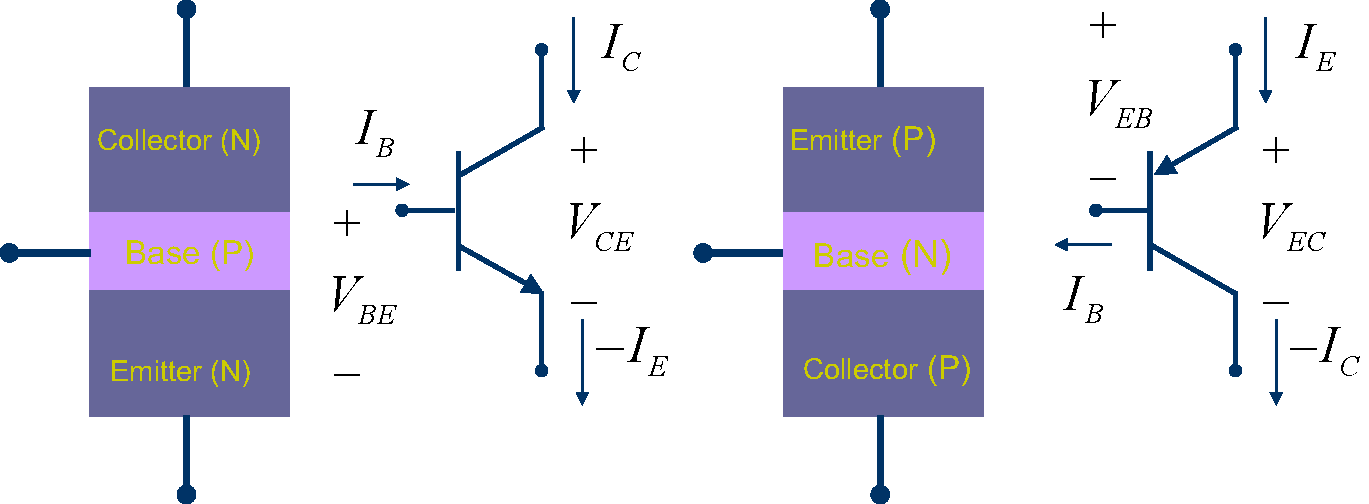
\includegraphics[width=.85\columnwidth]{slide2_bjt_overview}
\caption{Simplified device structure and schematic symbols for $NPN$ and $PNP$ bipolar junction transistors.}
\label{fig:slide2_bjt_overview}
\end{figure}
%%%%%%%%%%%%%%%%%%%%%%%%%%%%%%%%%%%%%%%%%%%%
The structure of a BJT transistor is deceptively simple.  It is just either an npn sandwich, or a pnp sandwich, as shown in \emph{Fig.~\ref{fig:slide2_bjt_overview}}.  Each region is a doped semiconductor, either $N$-type or $P$-type.  The middle part is the Base (B), and in an npn transistor (similar to NMOS), it's doped $P$-type.  Usually a bias voltage is applied across the npn transistor terminals in such a manner such that the top is at a positive voltage and the bottom at a lower voltage, sometimes ground.  The bottom is known as the Emitter (E), as it emits electrons into the base.  The electrons are "collected" at the Collector (C), at the top terminal.  So the current into the collector ideally flows out of the emitter, similar to an MOS device.
%%%%%%%%%%%%%%%%%%%%%%%%%%%%%%%%%%%%%%%%%%%%
But how does current flow at all, since the structure is two back-to-back diodes, pointing in opposite directions.  One diode says "one way" North and the other says "one way" South!  The two junctions cannot be simultaneously forward biased if the collector is at a high voltage relative to the base, which is the normal operating point for the transistor.  The solution lies in making the base very thin so that as minority carriers diffuse across the base from a forward biased base-emitter junction, they quickly reach the base-collector junction, where they are swept into collector due to the fields from the reverse biased junction, providing a pathway for current to flow.  
%%%%%%%%%%%%%%%%%%%%%%%%%%%%%%%%%%%%%%%%%%%%
In a well designed transistor, most of the emitter electron current flows into the collector and not the base, so 
    \begin{equation}
        {I_C} \approx  - {I_E}
    \end{equation}
and so the base current is very small:
    \begin{equation}
        {I_C} \gg {I_B}
    \end{equation}
And since the collector current is a forward-biased diode current of the base-emitter, it has the following form:
    \begin{equation}
        {I_C} \approx {I_S}{e^{\frac{{q{V_{BE}}}}{{kT}}}}
    \end{equation}
This behavior is very much a "transistor" one since the current through the collector is a function of another terminal-pair, namely the base-emitter.  Thus the BJT device is a voltage controlled current source, just like the MOS transistor.
%%%%%%%%%%%%%%%%%%%%%%%%%%%%%%%%%%%%%%%%%%%%
%             SUBSECTION 11.2.2            %
%%%%%%%%%%%%%%%%%%%%%%%%%%%%%%%%%%%%%%%%%%%%
\subsection{Actual BJT Cross-Section}
%%%%%%%%%%%%%%%%%%%%%%%%%%%%%%%%%%%%%%%%%%%%
%                 FIGURE                   %
%%%%%%%%%%%%%%%%%%%%%%%%%%%%%%%%%%%%%%%%%%%%
\begin{figure}[tb]
\centering
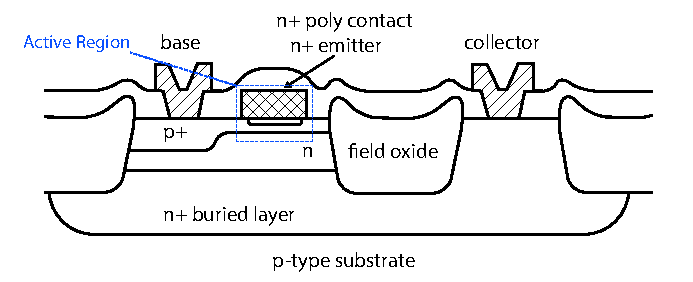
\includegraphics[width=.75\columnwidth]{slide3_bjtcross}
\caption{Cross-section of a BJT device fabricated in a planar process.  The actual transistor active region is under the emitter, with the p$^+$ base and n$^+$ buried layer providing low access resistance to the structure.}
\label{fig:slide3_bjtcross}
\end{figure}
%%%%%%%%%%%%%%%%%%%%%%%%%%%%%%%%%%%%%%%%%%%%
A real transistor is actually fabricated using a crystalline substrate with various layers grown using diffusion regions and counter-doping.  A typical "vertical" BJT is shown in \emph{Fig.~\ref{fig:slide3_bjtcross}}.  This is a complicated figure so let's dissect it piece by piece.   First let's focus in on the dashed box, the "active region" where the transistor actually resides.  This region is very much like the npn sandwich of an ideal structure.  The collector is the bottom $N$-type region, the middle region is a $P$-type base, and the top is made of an $N$-type emitter.  Notice that each layer is doped and so the concentration of dopants necessarily increases from the bottom to the top. The emitter is the most heavily doped, and the collector is the lightest doping. The base is in the middle in terms of doping.  This order, collector, then base, and then emitter is chosen for a good reason.  Due to symmetry, an $n_1 p n_2$ transistor can be viewed as an upside down transistor with $n_2 p n_1$, but due to the difference in doping levels, this upside down transistor is not a good transistor, as we shall see.  
%%%%%%%%%%%%%%%%%%%%%%%%%%%%%%%%%%%%%%%%%%%%
%                 FIGURE                   %
%%%%%%%%%%%%%%%%%%%%%%%%%%%%%%%%%%%%%%%%%%%%
\begin{figure}[tb]
\centering
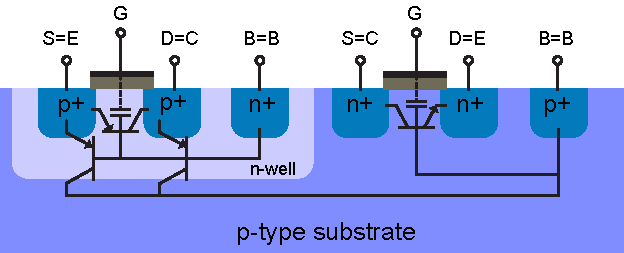
\includegraphics[width=.75\columnwidth]{mos_bjt}
\caption{Cross-section of a CMOS technology NMOS and PMOS devices.  Note that PMOS devices form lateral pnp transistors and substrate transistors.  Likewise NMOS devices form lateral npn devices with all bodies tied to the substrate.}
\label{fig:mos_bjt}
\end{figure}
%%%%%%%%%%%%%%%%%%%%%%%%%%%%%%%%%%%%%%%%%%%%
Transistors can also be fabricated laterally, similar to NMOS and PMOS devices.  In fact, if you examine the cross-section of a MOS device, such as \emph{Fig.~\ref{fig:mos_bjt}}, it actually has a couple of BJT's hiding in there!  Even though the gate couples capacitively to the channel, it can indirectly act like a base terminal.  These lateral BJTs tend to have inferior performance because the base width is determined lithographically rather than due to diffusion. One advantage of the BJT structure is in fact the ability to make very thin bases without using lithography, which in the early days was critical for good device performance.
%%%%%%%%%%%%%%%%%%%%%%%%%%%%%%%%%%%%%%%%%%%%
Everything else in the cross-section of the BJT is actually just there to support the device.  The n$^+$ buried layer is a low resistance contact to the collector, and the p$^+$ region under the base contact serves the same purpose.  The emitter is contacted using a highly doped polysilicon film. In fact, film can be used as the emitter itself.
%%%%%%%%%%%%%%%%%%%%%%%%%%%%%%%%%%%%%%%%%%%%
%             SUBSECTION 11.2.3            %
%%%%%%%%%%%%%%%%%%%%%%%%%%%%%%%%%%%%%%%%%%%%
\subsection{BJT Layout}
%%%%%%%%%%%%%%%%%%%%%%%%%%%%%%%%%%%%%%%%%%%%
%                 FIGURE                   %
%%%%%%%%%%%%%%%%%%%%%%%%%%%%%%%%%%%%%%%%%%%%
\begin{figure}[tb]
\centering
\subcaptionbox{\label{fig:slide4_bjt_layout}}{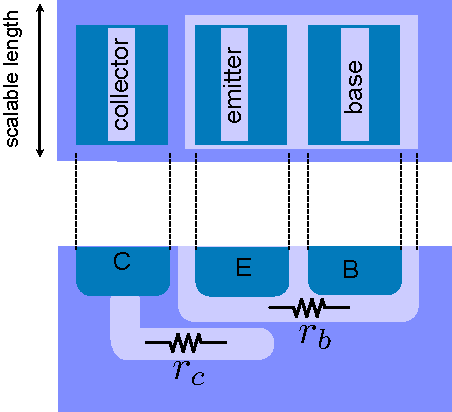
\includegraphics[width=.4\columnwidth]{slide4_bjt_layout}}
\hspace{1cm}
\subcaptionbox{\label{fig:bjt_round}}{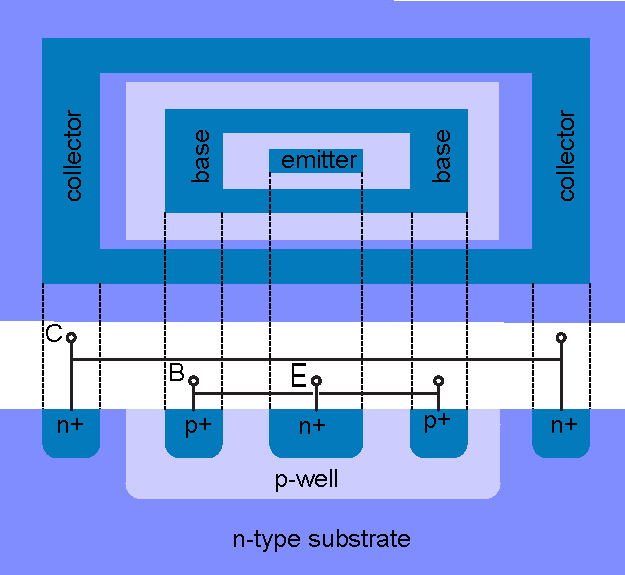
\includegraphics[width=.4\columnwidth]{bjt_npn_round}}
\caption{(a) A top view of a BJT transistor and corresponding cross-section.  The device is scaled by making it wider, or using multiple fingers of a basic device.  (b) Top view and cross-section of a BJT with rings of base and collector diffusion regions surrounding the device.} 
\end{figure}
%%%%%%%%%%%%%%%%%%%%%%%%%%%%%%%%%%%%%%%%%%%%
Let's now view the layout from the top, as shown in \emph{Fig.~\ref{fig:slide4_bjt_layout}}.  This is a unit cell that can grow in width as shown, similar to how we can scale a MOSFET.  The emitter area is the most relevant transistor parameter because the transistor current is injected from the emitter to the base.  The base and collector can also form rings around the device to lower the parasitic resistance (\emph{Fig.~\ref{fig:bjt_round}}).  Although it's not shown in this figure, a multi-finger layout strategy can be used to obtain lower parasitic resistances to the collector and base.  
%%%%%%%%%%%%%%%%%%%%%%%%%%%%%%%%%%%%%%%%%%%%
%             SUBSECTION 11.2.4            %
%%%%%%%%%%%%%%%%%%%%%%%%%%%%%%%%%%%%%%%%%%%%
\subsection{BJT Schematic Symbol}
%%%%%%%%%%%%%%%%%%%%%%%%%%%%%%%%%%%%%%%%%%%%
%                 FIGURE                   %
%%%%%%%%%%%%%%%%%%%%%%%%%%%%%%%%%%%%%%%%%%%%
\begin{figure}[tb]
\centering
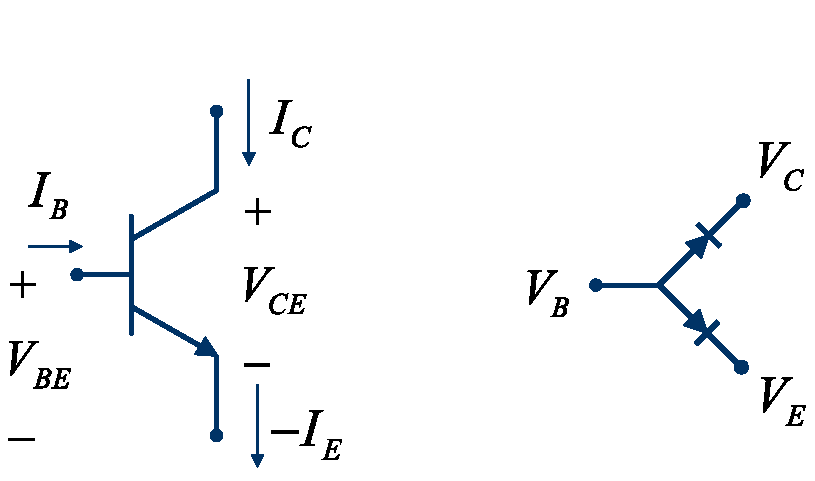
\includegraphics[width=.6\columnwidth]{slide5_bjt_schematic}
\caption{Definition of terminal currents (into the device) and junction voltages in a BJT.} \label{fig:slide5_bjt_schematic}
\end{figure}
%%%%%%%%%%%%%%%%%%%%%%%%%%%%%%%%%%%%%%%%%%%%
The schematic shown in \emph{Fig.~\ref{fig:slide5_bjt_schematic}} is for an npn device.  The symbol looks a lot like the MOSFET, and the arrow is in the direction of the base-emitter diode.  As already noted, the device looks symmetric but unlike a MOSFET the collector and emitter cannot be swapped because of the difference in doping profile. In fact, when the BJT is operated in this inverted fashion, it's in the "reverse active" regime and the performance is much worse as we shall explain shortly. 
%%%%%%%%%%%%%%%%%%%%%%%%%%%%%%%%%%%%%%%%%%%%%%%%%%%%%%%%%%%%%%%%%%%%%%%%%%%%%%%%%%%%%%%%
%%%%%%%%%%%%%%%%%%%%%%%%%%%%%%%%%%%%%%%%%%%%%%%%%%%%%%%%%%%%%%%%%%%%%%%%%%%%%%%%%%%%%%%%
%                                   SECTION 11.3                                       %
%%%%%%%%%%%%%%%%%%%%%%%%%%%%%%%%%%%%%%%%%%%%%%%%%%%%%%%%%%%%%%%%%%%%%%%%%%%%%%%%%%%%%%%%
%%%%%%%%%%%%%%%%%%%%%%%%%%%%%%%%%%%%%%%%%%%%%%%%%%%%%%%%%%%%%%%%%%%%%%%%%%%%%%%%%%%%%%%%
\section{Observed \texorpdfstring{$I-V$}{I-V} Characteristics}
In this section we will show typical $I$-$V$ curves of a BJT transistor, both in terms of a voltage control device and in terms of a current control device.  The first set of curves are similar to a MOSFET, but since only a bipolar transistor has base current, the second perspective is new.  One finds experimentally that the following equations describe the behavior of the device:
    \begin{equation}
        {I_C} = \beta_F {I_B}
    \end{equation}
    \begin{equation}
        {I_C} \approx {I_S}{e^{\frac{{q{V_{BE}}}}{{kT}}}}
    \end{equation}
These equations show that the collector current is an amplified copy of the base current.  Alternatively, in terms of voltages, the collector current is an exponential function of the base-emitter voltage.
%%%%%%%%%%%%%%%%%%%%%%%%%%%%%%%%%%%%%%%%%%%%
%             SUBSECTION 11.3.1            %
%%%%%%%%%%%%%%%%%%%%%%%%%%%%%%%%%%%%%%%%%%%%
\subsection{Base-Emitter Voltage Control}
%%%%%%%%%%%%%%%%%%%%%%%%%%%%%%%%%%%%%%%%%%%%
%                 FIGURE                   %
%%%%%%%%%%%%%%%%%%%%%%%%%%%%%%%%%%%%%%%%%%%%
\begin{figure}[tb]
\centering
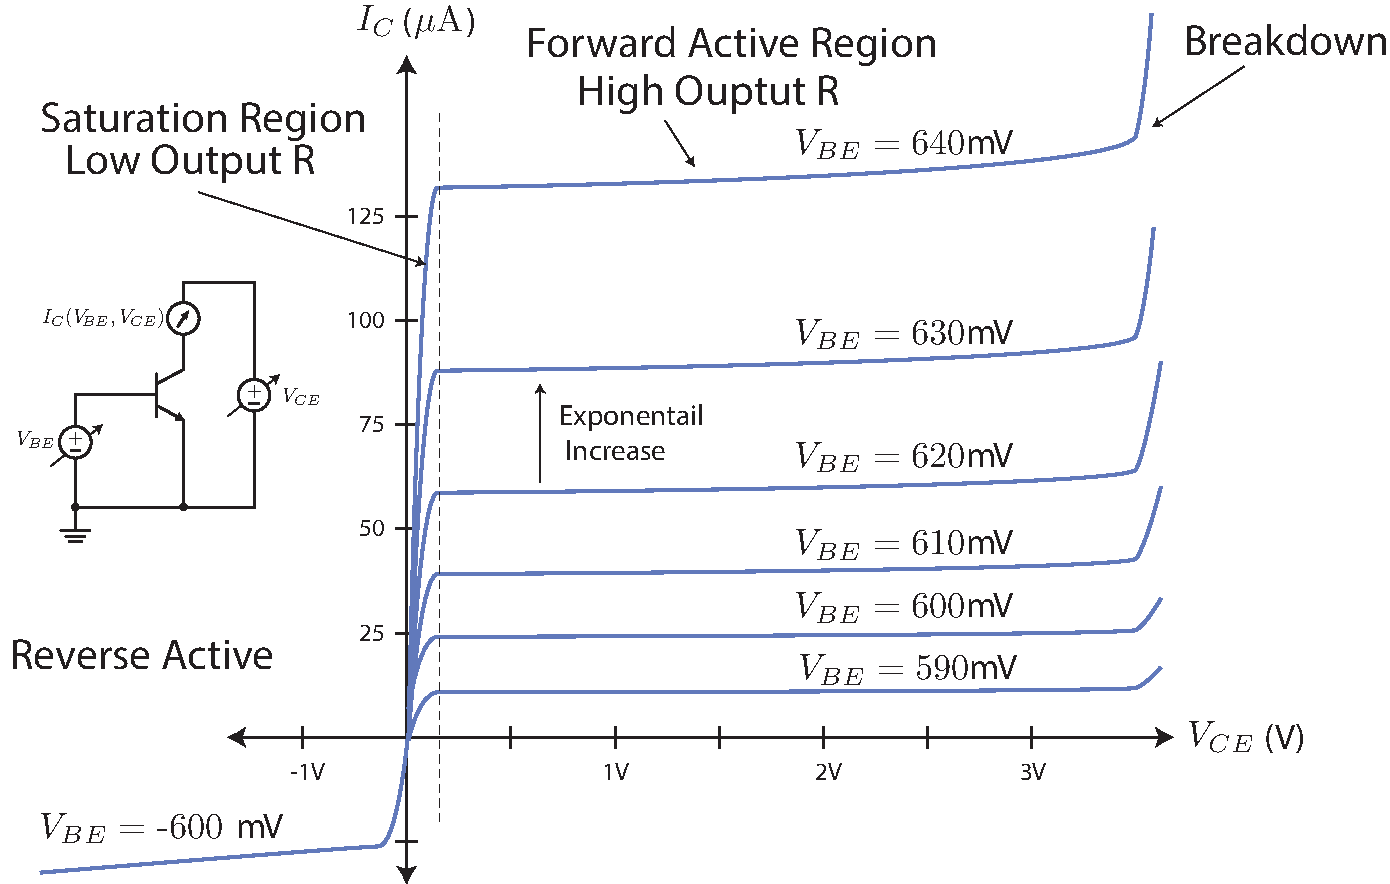
\includegraphics[width=\columnwidth]{slide8_bjt_ic_vs_ve_curves}
\caption{The $I_C$-$V_{BE}$ characteristics of an npn BJT transistor measured by sweeping the $V_{CE}$ voltage (x-axis) and observing the collector current $I_C$ (y-axis).  The family of curves are generated by varying the base voltage $V_{BE}$, as shown in the inset.  The current increases exponentially for linear changes in $V_{BE}$.}
\label{fig:slide8_bjt_ic_vs_ve_curves}
\end{figure}
%%%%%%%%%%%%%%%%%%%%%%%%%%%%%%%%%%%%%%%%%%%%
First let's observe the BJT device using voltage control on the base-emitter junction, as shown in the inset of \emph{Fig.~\ref{fig:slide8_bjt_ic_vs_ve_curves}}.  For a fixed $V_{BE}$, we sweep the collector-emitter voltage $V_{CE}$ to generate a $I_C$-$V_{CE}$ curve, and we observe that the current is approximately flat for a fixed value of $V_{BE}$.  As we increase $V_{BE}$ in discrete steps, we observe a family of curves with current increasing exponentially as we increase the base-emitter voltage linearly.  This is the diode $I$-$V$ curve we have met before.  What is curious about the transistor is that it's a diode between the base-emitter but the current can be collected at the collector rather than the base.
%%%%%%%%%%%%%%%%%%%%%%%%%%%%%%%%%%%%%%%%%%%%
%             SUBSECTION 11.3.2            %
%%%%%%%%%%%%%%%%%%%%%%%%%%%%%%%%%%%%%%%%%%%%
\subsection{Collector Characteristics \texorpdfstring{(Sweep $I_B$)}{}}
Now let's view the device as a current controlled device by grounding the emitter and applying a DC voltage $V_{CE}$.  Next we drive the base with a current $I_B$ and observe the collector current $I_C$.  The setup is shown in the inset of \emph{Fig.~\ref{fig:slide7_bjt_ic_vs_ib_curves}}, where we observe that in the \emph{forward active regime}, the BJT acts like a current controlled current source, with the collector current a much larger scaled copy of the base current.  This behavior is observed over a large range of $V_{CE}$ but if the collector voltage is dropped below a certain threshold, the device no longer behaves as a current source and the collector current drops rapidly.  What is happening is that in this region the collector-base junction is becoming forward biased and the device is no longer acting like a proper transistor. If the voltage is biased negatively, we enter the \emph{reverse active} region as discussed above.
%%%%%%%%%%%%%%%%%%%%%%%%%%%%%%%%%%%%%%%%%%%%
The key observation is that unlike a MOS device, the BJT has base current because the base is not insulated from the transistor like the gate of a MOSFET.  However, in a well designed transistor, this base current is a small fraction of the collector/emitter current.  Also, because of this base current and KCL, the collector and emitter currents cannot be identical, but they are nearly so.
%%%%%%%%%%%%%%%%%%%%%%%%%%%%%%%%%%%%%%%%%%%%
Now we must address a very confusing point about the nomenclature.  In a MOSFET the forward active region is also known as the \emph{saturation} region.  In a BJT, the region of low $V_{CE}$ is known as the \emph{saturation region}.  This is very confusing but it's common practice.
%%%%%%%%%%%%%%%%%%%%%%%%%%%%%%%%%%%%%%%%%%%%
Finally, all transistors have a maximum voltage that you can apply across the collector-emitter before they experience breakdown, or high currents.  The same behavior is observed in MOS devices.  
%%%%%%%%%%%%%%%%%%%%%%%%%%%%%%%%%%%%%%%%%%%%
%                 FIGURE                   %
%%%%%%%%%%%%%%%%%%%%%%%%%%%%%%%%%%%%%%%%%%%%
\begin{figure}[tb]
\centering
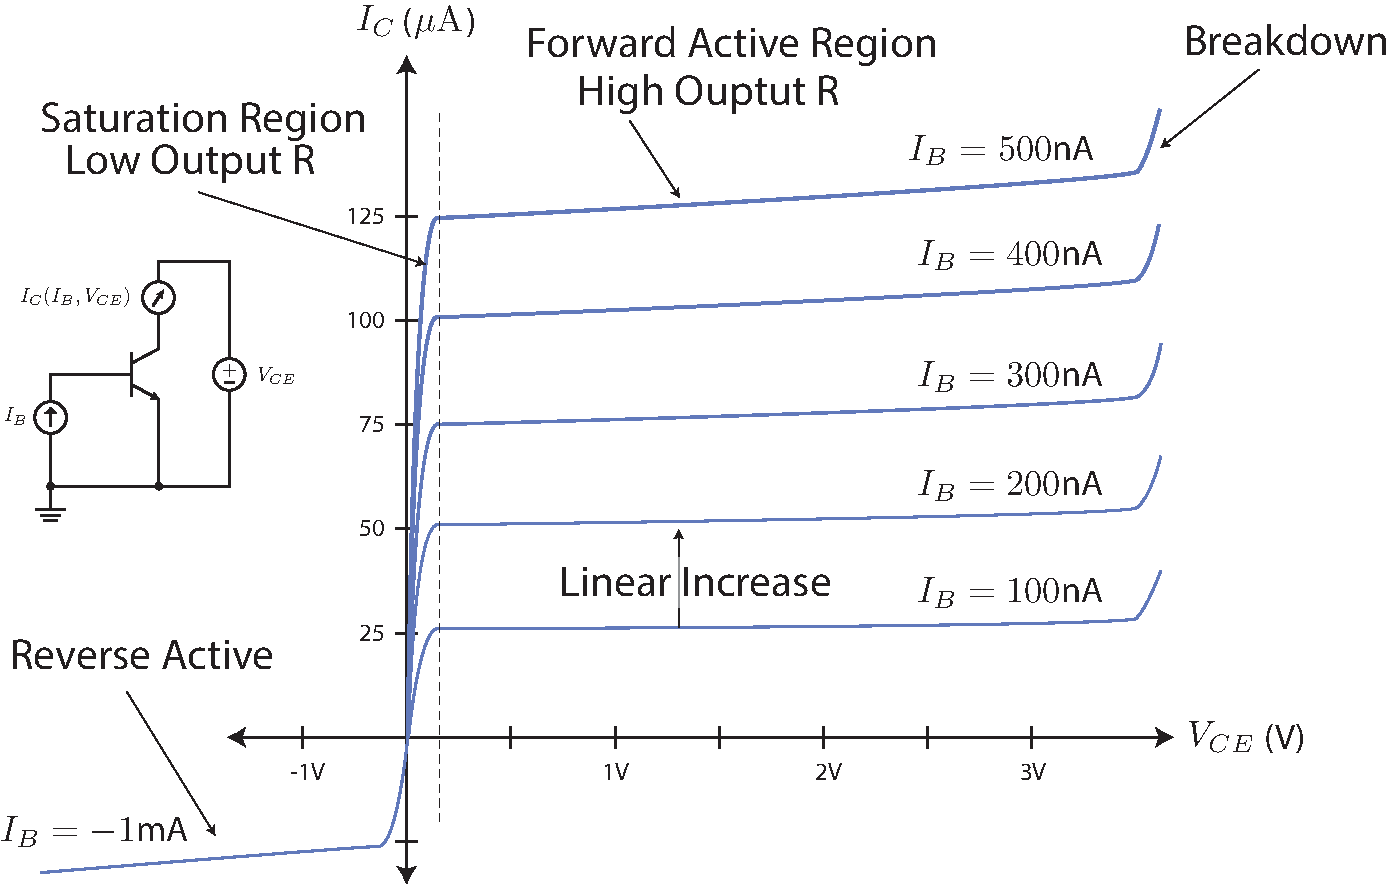
\includegraphics[width=.75\columnwidth]{slide7_bjt_ic_vs_ib_curves}
\caption{The $I_C$-$V_{CE}$ characteristics of an npn BJT transistor measured by sweeping the $V_{CE}$ voltage (x-axis) and observing the collector current (y-axis).  The family of curves are generated by varying the base current $I_B$, as shown in the inset.  $I_C$ scales in proportion to $I_B$ linearly, with a current gain defined as $\beta_F$.}
\label{fig:slide7_bjt_ic_vs_ib_curves}
\end{figure}
%%%%%%%%%%%%%%%%%%%%%%%%%%%%%%%%%%%%%%%%%%%%%%%%%%%%%%%%%%%%%%%%%%%%%%%%%%%%%%%%%%%%%%%%
%%%%%%%%%%%%%%%%%%%%%%%%%%%%%%%%%%%%%%%%%%%%%%%%%%%%%%%%%%%%%%%%%%%%%%%%%%%%%%%%%%%%%%%%
%                                   SECTION 11.4                                       %
%%%%%%%%%%%%%%%%%%%%%%%%%%%%%%%%%%%%%%%%%%%%%%%%%%%%%%%%%%%%%%%%%%%%%%%%%%%%%%%%%%%%%%%%
%%%%%%%%%%%%%%%%%%%%%%%%%%%%%%%%%%%%%%%%%%%%%%%%%%%%%%%%%%%%%%%%%%%%%%%%%%%%%%%%%%%%%%%%
\section{BJT Physics \emph{without} Equations}
%%%%%%%%%%%%%%%%%%%%%%%%%%%%%%%%%%%%%%%%%%%%
%             SUBSECTION 11.4.1            %
%%%%%%%%%%%%%%%%%%%%%%%%%%%%%%%%%%%%%%%%%%%%
\subsection{Transistor Action}
%%%%%%%%%%%%%%%%%%%%%%%%%%%%%%%%%%%%%%%%%%%%
%                 FIGURE                   %
%%%%%%%%%%%%%%%%%%%%%%%%%%%%%%%%%%%%%%%%%%%%
\begin{figure}[tb]
\centering
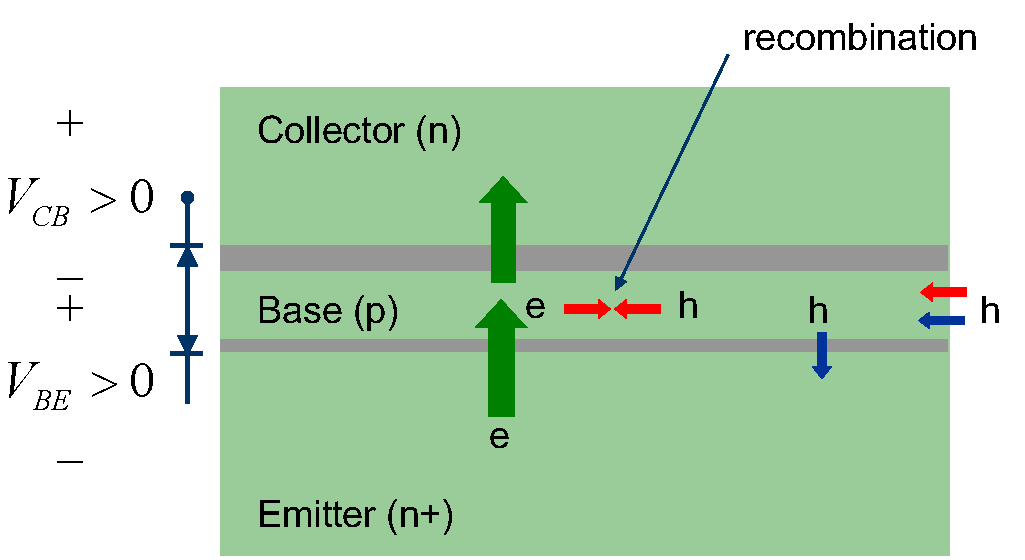
\includegraphics[width=.65\columnwidth]{slide9_bjt_action}
\caption{Schematic illustration of transistor action.  The large arrows show the injection of minority carriers (electrons for npn) into the base, and the subsequent diffusion into the collector region, where they are swept across the reverse-biased junction.  The smaller arrows are due to recombination and the correspondingly smaller minority carrier (holes for npn) injection from the base into the emitter.}
\label{fig:slide9_bjt_action}
\end{figure}
%%%%%%%%%%%%%%%%%%%%%%%%%%%%%%%%%%%%%%%%%%%%
How does a BJT transistor work its magic?   First let's assume that the transistor is in the forward active region, which means the base-emitter junction is forward biased and collector-base junction is reverse biased with respect to the base, or at a higher voltage than the base.  
%%%%%%%%%%%%%%%%%%%%%%%%%%%%%%%%%%%%%%%%%%%%
Since the base-emitter is a $PN$-junction, we know that in the forward bias it will inject electrons into the base due to diffusion, and likewise the base will inject holes into the emitter.  This is shown schematically in \emph{Fig.~\ref{fig:slide9_bjt_action}}.  Note that the "electron arrow" is larger than the "hole arrow" because the emitter is heavily doped compared to the base.  Now electrons in the base region can meet two fates:  They can either cross the base junction and be swept into the collector, or they might recombine with a hole in the base.  If the base width is much smaller than the diffusion length of minority carriers in the base, then it's more likely for the electrons to reach the collector, where they are collected, forming the collector current $I_C$.  If most of the emitted electrons are collected in this fashion, $I_C \approx I_E$.  
%%%%%%%%%%%%%%%%%%%%%%%%%%%%%%%%%%%%%%%%%%%%
The base current consists of the hole current injected into the emitter and the hole current to support the unlucky but rare electron-hole recombination.  
%%%%%%%%%%%%%%%%%%%%%%%%%%%%%%%%%%%%%%%%%%%%
%             SUBSECTION 11.4.2            %
%%%%%%%%%%%%%%%%%%%%%%%%%%%%%%%%%%%%%%%%%%%%
\subsection{Diffusion Currents}
%%%%%%%%%%%%%%%%%%%%%%%%%%%%%%%%%%%%%%%%%%%%
%                 FIGURE                   %
%%%%%%%%%%%%%%%%%%%%%%%%%%%%%%%%%%%%%%%%%%%%
\begin{figure}[tb]
\centering
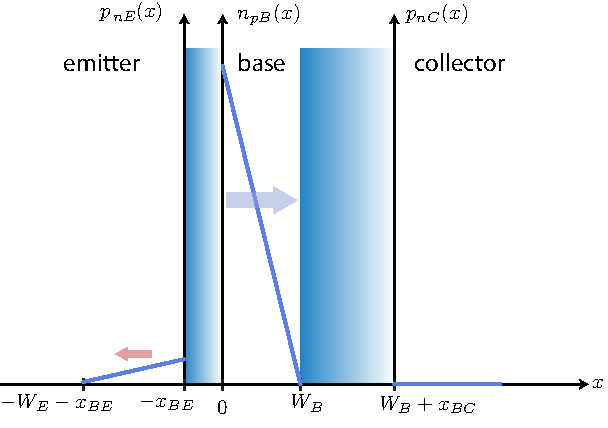
\includegraphics[width=.75\columnwidth]{slide10_minority_carriers}
\caption{Minority carrier profile in an npn transistor.  In this figure we assume negligible recombination, resulting in linear minority carrier profiles.}
\label{fig:slide10_minority_carriers}
\end{figure}
%%%%%%%%%%%%%%%%%%%%%%%%%%%%%%%%%%%%%%%%%%%%
A plot of the minority carriers in the various regions of a bipolar transistor are shown in \emph{Fig.~\ref{fig:slide10_minority_carriers}}.  The largest contribution to current is the minority carrier current in the base, in other words electrons injected from the emitter.  Also shown are the low concentration of holes in the emitter.  Once electrons are collected, they are no longer minority carriers and this is why the minority carrier concentration in the collector is not shown.  Here we are interested in gradients in the minority carrier concentration.
%%%%%%%%%%%%%%%%%%%%%%%%%%%%%%%%%%%%%%%%%%%%
%             SUBSECTION 11.4.3            %
%%%%%%%%%%%%%%%%%%%%%%%%%%%%%%%%%%%%%%%%%%%%
\subsection{BJT Currents}
As we have noted, the collector current is nearly identical to the (magnitude) of the emitter current 
    \begin{equation}
        {I_C} =  - {\alpha_F}{I_E}
    \end{equation}
where the factor $\alpha_F$  is a measure of the number of emitted electrons that are collected.  For example, if only 1 in a 1000 recombines in the base, we could say:
    \begin{equation}
        {\alpha _F} \sim .999
    \end{equation}
But by Kirchhoff's Law, for steady currents the sum of the currents into a transistor must sum to zero:
    \begin{equation} 
        - {I_E} = {I_C} + {I_B}
    \end{equation}
Using the relation between the emitter and collector currents,
    \begin{equation}
        {I_C} =  - {\alpha _F}{I_E} = {\alpha _F}({I_B} + {I_C})
    \end{equation}
allows us to find the DC current gain, or the $\beta_F$ of a transistor:
    \begin{equation}
        {I_C} = \frac{{{\alpha _F}}}{{1 - {\alpha _F}}}{I_B} = {\beta _F}{I_B}
    \end{equation}
Using values from our earlier calculation, we have
    \begin{equation}
        {\beta _F} = \frac{{{\alpha _F}}}{{1 - {\alpha _F}}} = \frac{{.999}}{{.001}} = 999
    \end{equation}
A good transistor is characterized by a high value of $\beta_F$.  In real transistors an absolute value of $\beta_F$ is never stated because it varies from device to device.  Instead, a range of values are given.  A typical $\beta_F =200$ is a good value to keep in mind. \emph{Never} design a circuit that relies on a particular value of $\beta_F$.  
%%%%%%%%%%%%%%%%%%%%%%%%%%%%%%%%%%%%%%%%%%%%
Electrons lost to recombination result in an exponentially decaying minority carrier profile, shown in \emph{Fig.~\ref{fig:slide12_alpha_f}}, and so the base current consists of both the recombination current and the forward biased  injection of holes into the emitter. 
%%%%%%%%%%%%%%%%%%%%%%%%%%%%%%%%%%%%%%%%%%%%
%                 FIGURE                   %
%%%%%%%%%%%%%%%%%%%%%%%%%%%%%%%%%%%%%%%%%%%%
\begin{figure}[tb]
\centering
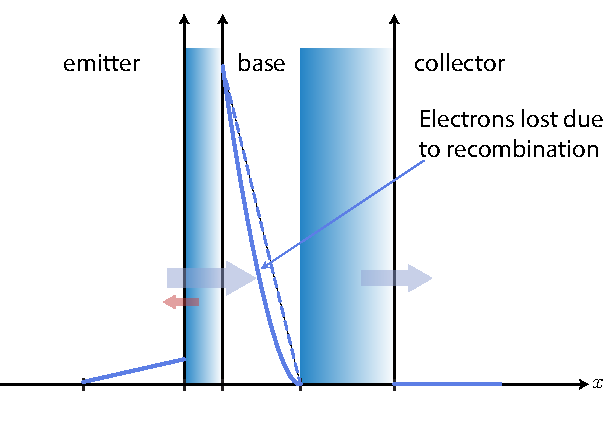
\includegraphics[width=.75\columnwidth]{slide12_alpha_f}
\caption{Minority carrier profile in an npn transistor.  In this figure we assume non-negligible recombination, resulting in an spatially decaying minority carrier profile in the base.  The base current is increased as a result, leading to a lower $\alpha_F$.}
\label{fig:slide12_alpha_f}
\end{figure}
%%%%%%%%%%%%%%%%%%%%%%%%%%%%%%%%%%%%%%%%%%%%%%%%%%%%%%%%%%%%%%%%%%%%%%%%%%%%%%%%%%%%%%%%
%%%%%%%%%%%%%%%%%%%%%%%%%%%%%%%%%%%%%%%%%%%%%%%%%%%%%%%%%%%%%%%%%%%%%%%%%%%%%%%%%%%%%%%%
%                                   SECTION 11.5                                       %
%%%%%%%%%%%%%%%%%%%%%%%%%%%%%%%%%%%%%%%%%%%%%%%%%%%%%%%%%%%%%%%%%%%%%%%%%%%%%%%%%%%%%%%%
%%%%%%%%%%%%%%%%%%%%%%%%%%%%%%%%%%%%%%%%%%%%%%%%%%%%%%%%%%%%%%%%%%%%%%%%%%%%%%%%%%%%%%%%
\section{BJT Device Physics \emph{with} Equations}
%%%%%%%%%%%%%%%%%%%%%%%%%%%%%%%%%%%%%%%%%%%%
%             SUBSECTION 11.5.1            %
%%%%%%%%%%%%%%%%%%%%%%%%%%%%%%%%%%%%%%%%%%%%
\subsection{Collector Current}
If you spent a great deal of time understanding the $PN$-junction device physics, it's about to pay off, because all the equations apply to the BJT.  The forward biased base-emitter junction results in a large diffusion of electrons across base:
    \begin{equation}
        J_n^{diff} = q{D_n}\frac{{d{n_p}}}{{dx}} = \left( {\frac{{q{D_n}{n_{pB0}}}}{{{W_B}}}} \right){e^{\frac{{q{V_{BE}}}}{{kT}}}}
    \end{equation}
Let's define the saturation current as
    \begin{equation}
        {I_S} = \left( {\frac{{q{D_n}{n_{pB0}}{A_E}}}{{{W_B}}}} \right)
    \end{equation}
which allows us to write the collector current in the following form:
    \begin{equation}
        {I_C} = {I_S}{e^{\frac{{q{V_{BE}}}}{{kT}}}}
    \end{equation}
%%%%%%%%%%%%%%%%%%%%%%%%%%%%%%%%%%%%%%%%%%%%
%             SUBSECTION 11.5.2            %
%%%%%%%%%%%%%%%%%%%%%%%%%%%%%%%%%%%%%%%%%%%%
\subsection{Base Current}
Since the base-emitter is forward biased, there's also a diffusion of holes into the emitter:
    \begin{equation}
        J_p^{diff} =  - q{D_p}\frac{{d{p_{nE}}}}{{dx}} = \left( {\frac{{q{D_p}{p_{nE0}}}}{{{W_E}}}} \right)\left( {{e^{\frac{{q{V_{BE}}}}{{kT}}}} - 1} \right)
    \end{equation}
Since all the holes arise from the base region, the base current is responsible for this component:
    \begin{equation}
        {I_B} = \left( {\frac{{q{D_p}{p_{nE0}}{A_E}}}{{{W_E}}}} \right)\left( {{e^{\frac{{q{V_{BE}}}}{{kT}}}} - 1}\right)
    \end{equation}
%%%%%%%%%%%%%%%%%%%%%%%%%%%%%%%%%%%%%%%%%%%%
%             SUBSECTION 11.5.3            %
%%%%%%%%%%%%%%%%%%%%%%%%%%%%%%%%%%%%%%%%%%%%
\subsection{Current Gain}
With equations for the base and collector current, we can find the transistor forward active current gain $\beta_F$:
    \begin{equation}
        {\beta _F} = \frac{{{I_C}}}{{{I_B}}} = \frac{{\left( {\frac{{q{D_n}{n_{pBo}}{A_E}}}{{{W_B}}}} \right)}}{{\left( {\frac{{q{D_p}{p_{nEo}}{A_E}}}{{{W_E}}}} \right)}} = \left( {\frac{{{D_n}}}{{{D_p}}}} \right)\left( {\frac{{{n_{pB0}}}}{{{p_{nE0}}}}} \right)\left( {\frac{{{W_E}}}{{{W_B}}}} \right)
    \end{equation}
Recall that we wish to maximize this term.  We can relate the minority carrier concentrations in the base and emitter to the doping concentrations:
    \begin{equation}
        \left( {\frac{{{n_{pB0}}}}{{{p_{nE0}}}}} \right) = \frac{{\frac{{n_i^2}}{{{N_{A,B}}}}}}{{\frac{{n_i^2}}	{{{N_{D,E}}}}}} = \frac{{{N_{D,E}}}}{{{N_{A,B}}}}
    \end{equation}
These equations tell us how to maximize the performance of the transistor.  We must dope the emitter as high as possible relative to the base, and the base width should be made as small as possible.  The physical reasons are clear and have already been discussed.  To recap, a short base width results in a high fraction of minority carriers flowing from the emitter to the collector.  A higher emitter doping results in more electron injection (diffusion) from the emitter side rather than hole injection (diffusion) from the base side, which also results in a relatively larger current $I_C$ compared to $I_B$.
%%%%%%%%%%%%%%%%%%%%%%%%%%%%%%%%%%%%%%%%%%%%%%%%%%%%%%%%%%%%%%%%%%%%%%%%%%%%%%%%%%%%%%%%
%%%%%%%%%%%%%%%%%%%%%%%%%%%%%%%%%%%%%%%%%%%%%%%%%%%%%%%%%%%%%%%%%%%%%%%%%%%%%%%%%%%%%%%%
%                                   SECTION 11.6                                       %
%%%%%%%%%%%%%%%%%%%%%%%%%%%%%%%%%%%%%%%%%%%%%%%%%%%%%%%%%%%%%%%%%%%%%%%%%%%%%%%%%%%%%%%%
%%%%%%%%%%%%%%%%%%%%%%%%%%%%%%%%%%%%%%%%%%%%%%%%%%%%%%%%%%%%%%%%%%%%%%%%%%%%%%%%%%%%%%%%
\section{Large Signal and Small-Signal Equivalent Circuits}
%%%%%%%%%%%%%%%%%%%%%%%%%%%%%%%%%%%%%%%%%%%%
%             SUBSECTION 11.6.1            %
%%%%%%%%%%%%%%%%%%%%%%%%%%%%%%%%%%%%%%%%%%%%
\subsection{Ebers-Moll Model}
We can now use some symmetry arguments and include both reverse and forward biased diode currents into the collector and emitter.   Recall that $\alpha_F$ represents the fraction of emitter carriers that reach the collector.  Likewise, when the transistor is biased in reverse active mode, $\alpha_R$ represents the fraction of injected carriers "collected" at the emitter side.  Combining these equations results in the \emph{Ebers-Moll Equations}:
    \begin{equation}
        {I_E} =  - {I_{ES}}\left( {{e^{{qV_{BE}}/{kT}}} - 1} \right)\, + {\alpha _R}{I_{CS}}\left( {{e^{{qV_{BC}}/{kT}}} - 1} \right)
    \end{equation}
The first term is the emitter diode current that we have been discussing, with the reverse minority carrier current included.  The current is negative because the diode is forward biased.  The second term is simply the reverse active current, and $\alpha_R$ represents the fraction of carriers that reach the emitter (rather than recombining) and is only significant if $V_{BC}$ is forward biased.  Under normal conditions, $V_{BC}$ is negative and the second term contributes only a small amount of current.  

Likewise, for the collector, we have the following symmetric relations:
    \begin{equation}
        {I_C} = {\alpha _F}{I_{ES}}\left( {{e^{{qV_{BE}}/{kT}}} - 1} \right) - {I_{CS}}\left( {{e^{{qV_{BC}}/{kT}}} - 1} \right)
    \end{equation}
It can be shown that the forward active and reverse active regions have a reciprocity relationship that dictates 
    \begin{equation}
        {\alpha _F}{I_{ES}} = {\alpha _R}{I_{CS}}
    \end{equation}
%%%%%%%%%%%%%%%%%%%%%%%%%%%%%%%%%%%%%%%%%%%%
%             SUBSECTION 11.6.2            %
%%%%%%%%%%%%%%%%%%%%%%%%%%%%%%%%%%%%%%%%%%%%
\subsection{Ebers-Moll Equivalent Circuit}
%%%%%%%%%%%%%%%%%%%%%%%%%%%%%%%%%%%%%%%%%%%%
%                 FIGURE                   %
%%%%%%%%%%%%%%%%%%%%%%%%%%%%%%%%%%%%%%%%%%%%
\begin{figure}[tb]
\centering
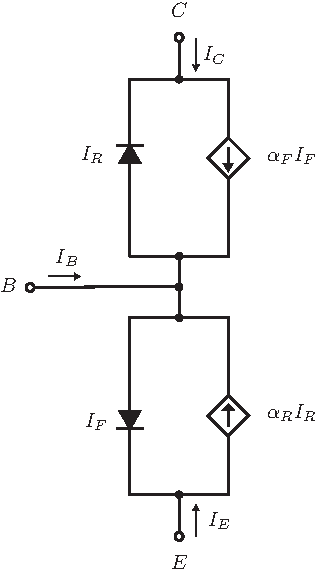
\includegraphics[scale=.7]{slide17_ebers_moll}
\caption{The large-signal Ebers-Moll circuit model of a BJT transistor.}
\label{fig:slide17_ebers_moll}
\end{figure}
%%%%%%%%%%%%%%%%%%%%%%%%%%%%%%%%%%%%%%%%%%%%
The Ebers-Moll equations are large-signal relations between the BJT transistor junction voltages and the resulting currents.  A physical model of the Ebers-Moll equations is shown in \emph{Fig.~\ref{fig:slide17_ebers_moll}}.  Note that each junction is represented by a diode, the forward diode $I_F$ and the reverse diode $I_R$.  When current flows through $I_F$, a fraction $\alpha_F I_F$ flows into the collector by the action of the controlled current source.  This is the normal forward active region. The base current is the difference current, and the reverse-biased diode current flow through $I_R$.  The model is totally symmetric, so if we interchange the role of the collector and emitter, the same physics should apply, but the currents will be different.  
%%%%%%%%%%%%%%%%%%%%%%%%%%%%%%%%%%%%%%%%%%%%
%             SUBSECTION 11.6.3            %
%%%%%%%%%%%%%%%%%%%%%%%%%%%%%%%%%%%%%%%%%%%%
\subsection{Forward Active Region and the Early Effect}
We can simplify the equivalent circuit model in the forward active region by noting that $I_R$ carries very little current, since if the B-C junction is reverse-biased, $I_R$ is very small and can be neglected.  So we can practically neglect $I_R$ and the controlled source that depends on it, resulting in the simpler model shown in \emph{Fig.~\ref{fig:slide18_ebers_moll_approx}}.
%%%%%%%%%%%%%%%%%%%%%%%%%%%%%%%%%%%%%%%%%%%%
With this approximation, we can write the collector current as
    \begin{equation}
        I_C = \alpha_F I_{ES} \left( e^{qV_{BE}/kT} -1 \right)
    \end{equation}
In practice this equation is modified to account for the non-zero output conductance of the device:
    \begin{equation}
        I_C = \alpha_F I_{ES} \left( e^{qV_{BE}/kT} -1 \right) \left( 1 + \frac{V_{CE}}{V_A} \right)
    \end{equation}
where $V_A$ is known as the Early Voltage, as introduced in Section~\ref{sec:mos_clm}.  In the MOSFET, increasing the drain-source voltage in saturation resulted in a larger depletion region width on the drain side, and this made the channel effectively shorter.  In a BJT, we have a similar effect, in that an increase in collector-emitter voltage results in a larger depletion region width on the base-collector junction, which shortens the base width, increasing the current.
%%%%%%%%%%%%%%%%%%%%%%%%%%%%%%%%%%%%%%%%%%%%
%                 FIGURE                   %
%%%%%%%%%%%%%%%%%%%%%%%%%%%%%%%%%%%%%%%%%%%%
\begin{figure}[tb]
\centering
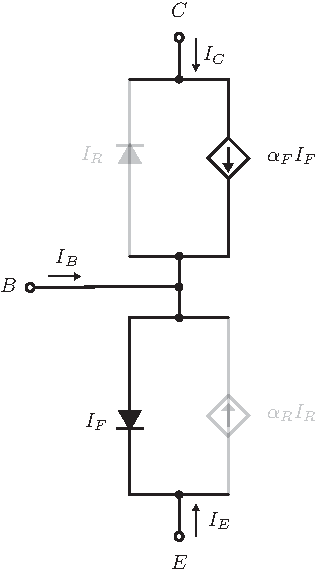
\includegraphics[scale=.7]{slide18_ebers_moll_approx}
\caption{The large-signal Ebers Moll circuit model of a BJT transistor in the forward active region.  The grayed out portions of the circuit can be neglected in the forward active region.} \label{fig:slide18_ebers_moll_approx}
\end{figure}
%%%%%%%%%%%%%%%%%%%%%%%%%%%%%%%%%%%%%%%%%%%%
%             SUBSECTION 11.6.4            %
%%%%%%%%%%%%%%%%%%%%%%%%%%%%%%%%%%%%%%%%%%%%
\subsection{Simplified Ebers-Moll}
Even simpler models are shown in \emph{Fig.~\ref{fig:slide19}}. The forward biased diode is treated as a battery with on-voltage of about 0.7V, and the collector current is simply an amplified version of the base current.  The model degenerates into two voltage sources in saturation, as both junctions are forward biased, with $V_{CE,sat}$ given by the difference between the diode on-voltages, shown in \emph{Fig.~\ref{fig:slide19}(b)}.
%%%%%%%%%%%%%%%%%%%%%%%%%%%%%%%%%%%%%%%%%%%%
%                 FIGURE                   %
%%%%%%%%%%%%%%%%%%%%%%%%%%%%%%%%%%%%%%%%%%%%
\begin{figure}[tb]
\centering
\subcaptionbox{\label{fig:slide19_model_fwd_active}}{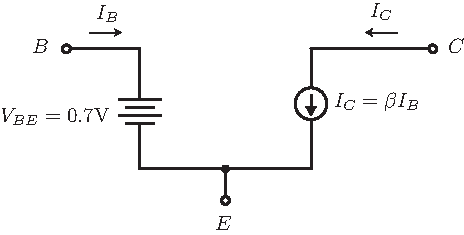
\includegraphics[scale=.7]{slide19_model_fwd_active}}
\subcaptionbox{\label{fig:slide19_model_sat}}{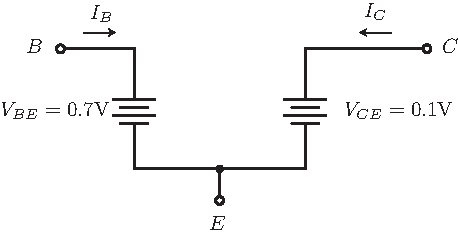
\includegraphics[scale=.7]{slide19_model_sat}}
\caption{Extremely simple models for a BJT device in the (a) forward active and (b) saturation region.} \label{fig:slide19}
\end{figure} 
%%%%%%%%%%%%%%%%%%%%%%%%%%%%%%%%%%%%%%%%%%%%
%             SUBSECTION 11.6.5            %
%%%%%%%%%%%%%%%%%%%%%%%%%%%%%%%%%%%%%%%%%%%%
\subsection{Small-Signal Model}
%%%%%%%%%%%%%%%%%%%%%%%%%%%%%%%%%%%%%%%%%%%%
%                 FIGURE                   %
%%%%%%%%%%%%%%%%%%%%%%%%%%%%%%%%%%%%%%%%%%%%
\begin{figure}[tb]
\centering
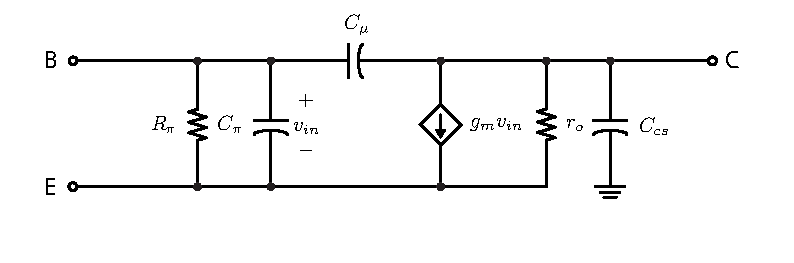
\includegraphics[scale=1]{bjt_hybridpi}
\caption{The Hybrid-$\Pi$ small-signal equivalent circuit model of a BJT transistor.} \label{fig:bjt_hybridpi}
\end{figure}
%%%%%%%%%%%%%%%%%%%%%%%%%%%%%%%%%%%%%%%%%%%%
The Ebers-Moll models are useful for DC calculations.  For most AC circuits, we make use of the equivalent circuit model, known as the hybrid-$\pi$ model, shown in \emph{Fig.~\ref{fig:bjt_hybridpi}}.  The model is very similar to the small-signal model of 3-terminal MOSFET, with one notable exception.  There is a resistance $R_\pi$ between the base and emitter because unlike a MOSFET, there's a current path for the base current.  
%%%%%%%%%%%%%%%%%%%%%%%%%%%%%%%%%%%%%%%%%%%%
It is not very difficult to show that the transconductance of the transistor is given by
    \begin{equation}
        g_m = \left. \frac{\partial I_C}{\partial V_{BE}} \right|_Q =  \frac{qI_C}{kT}
    \end{equation}
which is interesting to compare to a MOSFET.  For the MOSFET we showed (see \emph{Eq.~\ref{eq:gm_vstar}})
    \begin{equation}
        g_{m,\text{MOSFET}} = \frac{2 I_D}{V_{GS} - V_T}
    \end{equation}
For a fixed bias current $I_C = I_D$, the transconductance of a BJT is generally much higher because when biased in the strong inversion, $V_{GS} - V_T \gg kT/q$.  Recall that $kT/q$ is about 26mV at room temperature, and MOS devices in strong inversion are biased with several 100's of mV of overdrive.  In fact, if we try to reduce $V_{GS}-V_T$ to boost the transconductance, we are in fact biasing a MOS device as a BJT!  The trade-off is that the CMOS device is much slower in sub-threshold region.  This is why it's important to understand BJT device physics, even in a CMOS world.
%%%%%%%%%%%%%%%%%%%%%%%%%%%%%%%%%%%%%%%%%%%%
The transistor base resistance $R_\pi$ is given by
    \begin{equation}
        R_\pi^{-1} = \left. \frac{\partial I_B}{\partial V_{BE}} \right|_Q = \frac{1}{\beta_F} \left. \frac{\partial I_C}{\partial V_{BE}}  \right|_Q = \frac{g_m}{\beta_F}
    \end{equation}
    \begin{equation}
        R_\pi = \frac{\beta_F}{g_m}
    \end{equation}
This makes sense since the base current is $\beta_F$ times smaller than the collector current.  The resistor $r_o$ models the device output resistance: 
    \begin{equation}
        r_o^{-1} = \left. \frac{\partial I_C}{\partial V_{CE}} \right|_Q  = \frac{I_C}{V_A}
    \end{equation}
    \begin{equation}
        r_o = \frac{V_A}{I_C}
    \end{equation}
Since the base-emitter and base-collector are $PN$-junctions, there's an associated junction capacitance.  In forward active region, $C_{\mu} = C_{j,bc}(V_{BC})$ is the base-collector reverse biased junction capacitance.  Likewise $C_\pi$ contains the forward-biased junction capacitance, but also models the minority charge storage effects we discussed when we analyzed the diode, see Section~\ref{sec:charge_storage}:
    \begin{equation}
        C_\pi \approx 1.4 C_{j,be0} + C_{diff}
    \end{equation}
The factor 1.4 models the increase in junction capacitance under forward bias.  The diffusion capacitance is given by a similar expression we presented for a diode:
    \begin{equation}
        C_{diff} = g_m \tau_F 
    \end{equation}
The factor $\tau_F$ is a technology parameter known as the "forward transit time" and it's essentially the time it takes a minority carrier to cross the various regions and junction.  The physical reason for this is that charge is stored in the base due to the minority carrier diffusion profile in the base.  If the base current is increased, it takes a finite amount of time to build a new diffusion profile, a time that corresponds to how long it takes for minority carriers to flow into the base.
